\section{Réseau, configuration classique: machines derrière une \og
  box\fg}

\begin{center}
  \begin{minipage}{0.6\textwidth}
    \textsl{Ce qui suit n'est pas propre à Linux, ni à Unix, bien sûr.
      La deuxième partie (commandes Linux, page \pageref{netlinux}),
      elle, est spécifique à Unix 
      (Linux).} 
  \end{minipage}
\end{center}
\begin{figure}
  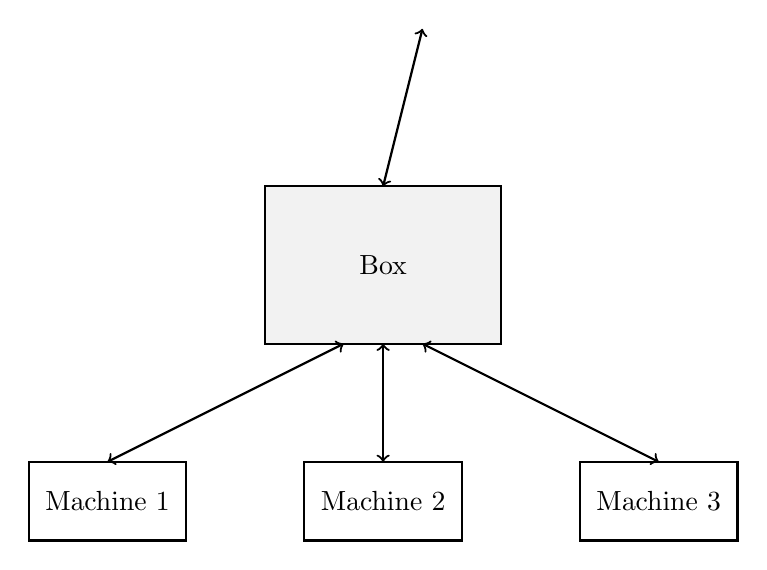
\begin{tikzpicture}[level distance=10mm,thick]
    \draw (3,5) rectangle +(3,2) [fill=gray!10]  node[midway]
          {Box};
          
          \draw[<->] (4.5,7)--(5,9);

    \draw (0,2.5) rectangle +(2,1)  node[midway]
          {Machine 1};
          \draw[<->] (1.,3.5)--(4,5);
          
    \draw (3.5,2.5) rectangle +(2,1)  node[midway]
          {Machine 2};
          \draw[<->] (4.5,3.5)--(4.5,5);
          
    \draw (7,2.5) rectangle +(2,1)  node[midway]
          {Machine 3};
          \draw[<->] (8,3.5)--(5,5);
    
  \end{tikzpicture}
  \caption{machines derrière une  \og   box\fg}\label{box}
\end{figure}

\subsection{Le cas \og classique\fg{}: IPv4}
Toute machine a une adresse, qui en IPv4 est de la forme (par
exemple): 134.214.100.121 et chaque adresse est unique. Les 4 nombres
qui forment l'adresse sont stockés chacun sur un octet ce qui
correspond à des nombres compris entre $0$ et $255$
(bornes incluses)\footnote{Car $255 = 1+2 +4+\ldots+2^7 = 2^8 -1$.}. L'adresse
IPv4 est donc stockée sur 32 bits (4 octets) et le nombre d'adresses
disponibles est donc de $2^{32} -1= 4294967295$ soit un peu plus de 4
milliards d'adresses. Sachant que, comme on va le voir, certaines
adresses sont réservées à des usages particuliers, c'est peu et
actuellement insuffisant. IPv4 peut donc être considéré comme un
protocole en fin de vie.

La technique utilisée derrière les  \og   box\fg{} est celle du
\emph{réseau local} (voir figure \ref{box}): seule la  \og   box\fg{}
est visible du monde extérieur, possède une adresse ip connue de
l'internet.

Les machines situées derrière ont des adresses qui sont invisibles du
monde extérieur forment un réseau local:

\begin{itemize}
  \item les machines du sous réseau local: elles  ont des adresses
    comprises entre 
  192.168.0.0 et 192.168.255.0. Ces adresses ne sont certainement pas
  uniques, mais sont invisibles de l'internet. La \og box\fg{} agit
    comme un barrage, laissant quand même passer ce qui est nécessaire.

\end{itemize}
Cela pose un certain nombre de questions:
\begin{enumerate}

\item Comment sont affectées
  les adresses aux machines du réseau local? à ma \og box\fg?
\item Comment les machines du réseau local
  communiquent-elles avec le mode extérieur?
\item Comment fait-on pour joindre une machine extérieure eu réseau
  local, connaissant son nom?
\end{enumerate}

Et bien sûr quels sont les outils Linux (Unix) associés, quelles sont
les commandes qui permettent d'explorer ce fonctionnement?

Auparavant il faut comprendre un peu comment fonctionne IP (v4 dans ce
cas).
\subsection{Internet protocol}
Un paquet IP est formé d'une en-tête et de données. L'en-tête est
décrite à la figure \ref{entetev4}. Pour une description détaillée,
consulter par exemple \cite{v4}. Parmi les champs de l'en-tête,
retenons:
\begin{itemize}
  \item Adresse source (32 bits):
    adresse IP de l'émetteur sur 32 bits.
  \item Protocole (8 bits):
    numéro du protocole au-dessus de la couche réseau : TCP = 6, UDP =
    17, ICMP = 1.
   \item Identification (16 bits):
    Numéro permettant d'identifier les fragments d'un même paquet.
\end{itemize}
\begin{figure}
  \includegraphics[width=0.8\textwidth]{images/entetev4.png}
  \caption{En-tête IPv4}\label{entetev4}
\end{figure}
\subsection{Le NAT (Network Adress Translation}
Supposons que la machine 1 (figure \ref{box}) veuille envoyer un
paquet à l'extérieur. La box (un système Linux, à priori) va changer
l'adresse ip (192.....) de la machine 1 par sa propre adresse, et se
souvenir d'un identifiant unique du paquet. Au retour, il enverra le
paquet de retour vers la machine 1 (C'est un peu simplifié). Donc, de
l'extérieur, on ne voit que la \og box\fg.

Comment tester ça? Il suffit d'aller sur le site
\url{https://www.whatismyip.com/fr/}: si vous avez plusieurs machines
dans votre réseau local (ordinateur, téléphone sur le wi-fi, etc.)
quelque soit la machine que vous utiliserez pour consulter cette url,
vous obtiendrez la même adresse v4.

Bien mais ceci ne nous dit pas:
\begin{enumerate}
\item Comment chaque machine du réseau local connaît-elle les
    paramètres nécessaires à son fonctionnement (entre autres son adresse ip)?
  \item Comment la box sait-elle faire la différence entre un trafic
    local et un accès vers l'extérieur?
  \item Comment associer un nom (exemple: \ttt{www.aldil.org}) à une
    adresse ip et vice versa?
\end{enumerate}


\subsubsection{La configuration réseau de la machine}
Jadis, on faisait ça à la main en remplissant un fichier. Pas très
facile, ni pratique pour un portable appelé à changer de réseau.

C'est un service: une machine dans le réseau (c'est la
box, mais ce peut être une autre) fait tourner un démon \ttt{DHCP}.
De façon sommaire: la machine en manque de configuration envoie un
paquet IP en \emph{broadcast} (à la cantonade! --voir plus bas--). Le
paquet contient 
entre autres l'\emph{adresse MAC} de la machine \emph{cliente}. Le
serveur \ttt{DHCP} envoie alors tous les renseignements nécessaires à
la configuration réseau de la machine cliente, dont son adresse IP (il 
se base sur l'adresse MAC, pour lui associer une adresse
IP\footnote{Plusieurs méthodes sont possibles: adresse IP dans une
  table (l'adresse de la machine est alors fixe), ou tirage
  aléatoire.}; il envoie aussi tous les autres paramètres dont la
machine a (ou peut avoir) besoin
(voir \cite{dhcp} pour une explication un peu détaillée).
\subsubsection{l'adresse MAC} est un identifiant unique d'une
interface réseau: c'est attribué à la construction, et c'est à priori
unique. Exemple:

\ttt{d8:50:e6:ba:2e:d8 brd ff:ff:ff:ff:ff:ff}


\subsubsection{Que faire des paquets qui ne sont pas destinés à une
  machine locale?} Il faut les envoyer à une machine qui fait office
de porte de sortie (GATEWAY). La machine du réseau local doit donc
connaître l'adresse IP de cette porte (ça fait partie des paramètres
renvoyés par le serveur DHCP). La machine GATEWAY a deux interfaces
réseau configurées:
\begin{enumerate}
  \item une sur le réseau local (celle que connaissent las machines du
    réseau local),
  \item une adresse sur le réseau extérieur (celui du FAI dans notre
    cas). C'est celle qu'on voit quand on va sur le site
    \url{https://www.whatismyip.com/fr/} par exemple.
\end{enumerate}
Dans notre cas, le GATEWAY, physiquement, c'est la box, mais ce n'est
pas obligatoire.
\subsubsection{Netmask (masque de sous-réseau)}
Supposons que mon adresse ip soit 51.75.22.226. Quelle sont les
adresses qui font partie du même sous-réseau que moi? Le sous-réseau
peut être mon réseau local privé derrière ma box, ou, disons le réseau
free.fr ou...?

Les adresses d'un même sous-réseau partagent un début d'adresse (partie
gauche) commune. On trouve en général la notation
192.168.0.10/24. Dans ce cas cela veut dire que les 24 premiers bits
en partant de la gauche sont communs aux adresses du réseau. Ici $24 =
3 \times 8$ et donc les adresses de l'ensemble  de réseau sont de la
forme 192.168.0.xyz. Le masque donne donc aussi la taille du
sous-réseau (127 adresses ici).

Toujours dans l'exemple ci-dessus, le nombre de 4 octets ayant 24 ses
bits de gauche à 1 et les autres à 0 s'écrit (en séparant les octets
par un ``.''): 

$$ 1111.1111.1111.0$$

et comme $1111 = 255$ en base 10, cela peut se noter:

$$255.255.255.0$$

qui est le \emph{netmask} du réseau.

Cela permet de répondre à la question suivante: étant donné une
adresse IPv4, est-elle dans le même réseau que moi? Là, il faut faire
un peu de logique: on assimile 0 à la valeur \emph{faux} et 1 à la
valeur \emph{vrai}. On a:

\begin{itemize}
\item 0 ET 0 = 0 (faux et faux est faux)
\item 0 ET 1 = 0 (faux et vrai est vrai)
\item 1 ET 0 = 0 (vrai et faux est faux)
\item 1 ET 1 = 1 (vrai et vrai est vrai).
\end{itemize}
 On fait un \og ET\fg{} bit à bit antre le netmask et l'adresse
 testée. Exemples
 \begin{itemize}
 \item 192.168.0.21, le netmask étant 255.255.255.0.

   $192.168.0.21$ est $11000000.10101000.00000000.00010101$ en
   binaire. Le netmask est $11111111.11111111.11111111.0$. Le ``ET''
   entre le netmask et mon adresse ip est
   
   $$11000000.10101000.00000000.0000000.$$
   
 \item Pour l'adresse 192.168.0.32, le calcul précédent donne le même
   résultat: les deux adresses sont donc dans le même réseau.
 \item Mais pour 134.214.100.8, le résultat est différent, et les deux
   adresses ne sont donc pas dans le même réseau.
\end{itemize}
   
 

\subsubsection{Adresse de broadcast}
Comment contacter toutes les machines du même réseau?

On considère la partie commune des adresses du réseau: dans mon cas,
utilisant le netmask 255.255.255.0, et mon adresse étant 192.168.0.32,
j'en déduis que les machines de mon réseau ont toutes des adresses de
la forme 192.168.0.x ou x est compris entre 0 et 255. L'adresse de
broadcast est obtenue en remplaçant ``x'' par des 1 en binaire, ce qui
ici donne

$$192.168.0.255.$$

Envoyer un paquet IP avec cette adresse de destinataire, c'est écrire
à toutes les machines du réseau.

\subsubsection{Serveur de noms (DNS, Domain Name System)}
La configuration réseau d'une machine contient au minimum 4
paramètres:
\begin{enumerate}
\item l'adresse IP,
\item le netmask,
\item l'adresse de la GATEWAY,
\item l'adresse du serveur de noms.
\end{enumerate}
Le \emph{serveur de noms} est chargé d'associer un nom
(\ttt{www.aldil.org} par exemple) à une adresse ip, et vice-versa.

Supposons que je cherche l'adresse de \ttt{math.univ-lyon1.fr}; le
fonctionnement est à peu près le suivant: 
\begin{enumerate}
  \item Est-ce que je connais l'adresse IP de
    \ttt{math.univ-lyon1.fr}? Si oui, c'est fini. Sinon, j'envoie une
    requête au serveur de nom précédemment défini.
  \item Est ce que le serveur de nom connaît l'adresse que je cherche?
    Dans mon cas le serveur de nom peut être un serveur qui tourne
    dans la box, ou bien je consulte celui de mon FAI, disons
    \ttt{free.fr}.
  \item Si le serveur de nom de \ttt{free.fr} connaît l'adresse du
    serveur de nom de \ttt{univ-lyon1.fr}, il lui demande l'adresse de
    \ttt{math.univ-lyon1.fr}; peut être faut-il une étape
    supplémentaire si  \ttt{univ-lyon1.fr} est inconnu chez
    \ttt{free.fr}: dans ce cas il consulte le DNS de \ttt{fr}, qui
    connaît obligatoirement \ttt{univ-lyon1.fr}.
  \item Une fois un serveur capable de répondre à notre requête
    atteint, celui envoie l'adresse IP, mais aussi une durée garantie
    de validité de cette adresse. Alors \emph{tous} les serveurs de nom
    et au bout votre machine elle-même vont se souvenir de ce renseignement, ce
    qui  permet de limiter le trafic sur le réseau.
    
\end{enumerate}
Évidemment les serveurs DNS contiennent des tables associant adresses
et noms.
\subsection{En résumé}
Pour IPv4, il faut au minimum  4 paramètres pour définir la
configuration réseau d'une machine:
\begin{itemize}
\item L'adresse de la machine.
\item Celle de la GATEWAY.
\item Celle du DNS.
\item Le netmask.
\end{itemize}
Pour une description plus détaillée consulter par exemple \cite{dns}.
\subsection{Ports} A chaque adresse IP on associe des ports, qui sont
des nombres entiers. Cela permet de séparer le trafic. Chaque protocole
est associé à un ou plusieurs ports. Par exemple le port 80 est
associé à \ttt{http}, et un serveur web écoutera à priori sur ce port.

Dans le cas de ma box, il est possible de \emph{router} un port donné
sur vers machine du réseau local, par exemple le port 80 sur la
machine 1\footnote{Ce qui restreint les possibilités: un seul serveur
  web  dans le réseau, par exemple.}.

\subsection{IPv6}
  Les adresses ne sont plus stockées sur 32 bits mais sur 128 bits (16
  octets).

  Petit calcul:

  \begin{itemize}
    \item le rayon $R$ de la terre est de 6000 kms environ, soit $6000
      \times 1000$ mètres. la surface de la terre donc environ (en
      mètres carrés) de
      $$S= 4 \pi R^2.$$
    \item Le nombre d'adresses IP v6 disponibles par mètre carré est
      donc environ:
      $$\frac{2^{128} }{4 \pi R^2},$$
      ce qui fait environ $7,5\times  10^{23}$ adresses au mètre
          carré\footnote{Comment je calcule ça? Avec SageMath:
            \url{https://www.sagemath.org/} et
            \url{http://sagebook.gforge.inria.fr/english.html}}!
  \end{itemize}

  La notation des adresses est un peu différente. Cela pourra être:

  \ttt{2001:0db8:0000:85a3:0000:0000:ac1f:8001}

  Pourquoi des lettres (\ttt{db}, \ttt{a})? Ces  adresses sont écrites
  en base 16 pour laquelle on note les chiffres
  $0,1,\ldots,9,a,b,c,d,e,f$ (15 chiffres), ce qui rend l'écriture plus
  compacte. Des écritures condensées existent, voir \cite{v6}.

  \subsubsection{Notes importantes}
  \begin{itemize}
    \item La migration vers v6 est en cours (v6 disponible chez
    free.fr et adopté en remplacement de v4 chez orange (peut-être
    seulement sur certaines parties du réseau?)).
    \item IPv4 et IPv6 forment deux réseaux différents qui peuvent
      communiquer par des passerelles.
    \item Il est bien évident qu'avec IPv6, le NAT disparaît. Chacune
      de vos machines, sont accessibles directement derrière votre
      box! (et tous les ports de toutes les machines peuvent à priori
      être accédées).
    \item Pour le netmask, rien de changé, on adapte juste à la
      longueur de l'adresse.
    \item Le DNS est adapté.
  \end{itemize}


    
